\documentclass[11pt,a4paper]{article}
\usepackage[margin=1in]{geometry}
\usepackage{amsmath,amsthm,amssymb}
\usepackage{graphicx}
\usepackage{hyperref}
\usepackage{natbib}
\usepackage{booktabs}

\newtheorem{theorem}{Theorem}
\newtheorem{proposition}{Proposition}
\newtheorem{definition}{Definition}

\title{\textbf{Topology-Performance Tradeoffs in Reservoir Computing:\\ Sparsity Optimization Across Dynamical Regimes}}

\author{Research Investigation}
\date{\today}

\begin{document}

\maketitle

\begin{abstract}
Reservoir computing has emerged as a powerful paradigm for time-series prediction, with Echo State Networks (ESNs) demonstrating remarkable performance across diverse applications. However, the relationship between reservoir topology—specifically connectivity sparsity—and prediction performance across different dynamical regimes remains poorly understood. This paper investigates how reservoir sparsity affects predictive capabilities for periodic, chaotic, and noisy time series. Through systematic computational experiments, we demonstrate that optimal sparsity levels are regime-dependent: chaotic systems benefit from denser connectivity (sparsity $\approx 0.15$), while periodic signals perform optimally with sparser topologies (sparsity $\approx 0.25$). We provide spectral analysis of optimal reservoir configurations and establish connections to memory capacity, revealing fundamental tradeoffs between computational efficiency and predictive power. Our findings offer practical guidelines for reservoir design and contribute to the theoretical understanding of how network topology shapes computational capabilities in recurrent neural systems.
\end{abstract}

\section{Introduction}

Reservoir computing \citep{jaeger2001echo, maass2002real} represents a paradigm shift in recurrent neural network training, where only the readout layer is trained while the recurrent dynamics remain fixed. This approach has proven remarkably effective for temporal pattern recognition, time-series prediction, and dynamical systems modeling \citep{lukosevicius2009reservoir}. Recent work by Hart and colleagues \citep{hart2021thesis, hart2022brain, hart2025hippocampal} has explored biological implementations and theoretical foundations of reservoir computing, highlighting the importance of network structure in computational performance.

Despite extensive research, a critical gap remains in understanding how reservoir topology—particularly connectivity sparsity—interacts with the dynamical characteristics of target systems. While conventional wisdom suggests that denser networks provide greater computational power, the reality is more nuanced. Sparse connectivity offers computational efficiency, biological plausibility, and potentially better generalization, but at what cost to predictive performance?

\subsection{Research Questions}

This paper addresses three interconnected questions:

\begin{enumerate}
    \item How does reservoir sparsity affect prediction performance across different dynamical regimes (periodic, chaotic, noisy)?
    \item What spectral properties characterize optimal reservoir configurations for each regime?
    \item How does sparsity influence memory capacity, and what implications does this have for reservoir design?
\end{enumerate}

\subsection{Contributions}

Our main contributions are:

\begin{itemize}
    \item \textbf{Empirical characterization} of sparsity-performance relationships across three distinct dynamical regimes
    \item \textbf{Spectral analysis} revealing regime-specific optimal network topologies
    \item \textbf{Memory capacity analysis} establishing fundamental tradeoffs in reservoir design
    \item \textbf{Practical guidelines} for selecting reservoir sparsity based on target system characteristics
\end{itemize}

\section{Background and Related Work}

\subsection{Echo State Networks}

An Echo State Network consists of three components: an input layer, a randomly connected reservoir, and a trained readout layer. The reservoir dynamics are governed by:

\begin{equation}
\mathbf{x}(t+1) = (1-\alpha)\mathbf{x}(t) + \alpha \tanh(\mathbf{W}\mathbf{x}(t) + \mathbf{W}_{in}\mathbf{u}(t))
\end{equation}

where $\mathbf{x}(t) \in \mathbb{R}^N$ is the reservoir state, $\mathbf{u}(t) \in \mathbb{R}^K$ is the input, $\alpha$ is the leak rate, $\mathbf{W} \in \mathbb{R}^{N \times N}$ is the reservoir weight matrix, and $\mathbf{W}_{in} \in \mathbb{R}^{N \times K}$ contains input weights.

The output is computed as:
\begin{equation}
\mathbf{y}(t) = \mathbf{W}_{out}\mathbf{x}(t)
\end{equation}

where $\mathbf{W}_{out}$ is trained using ridge regression to minimize prediction error.

\subsection{The Echo State Property}

For stable reservoir dynamics, the system must satisfy the \emph{echo state property} \citep{jaeger2001echo}: the reservoir state should asymptotically depend only on the input history, not on initial conditions. A sufficient condition is that the spectral radius $\rho(\mathbf{W}) < 1$, though this can be relaxed depending on input characteristics and activation functions.

\subsection{Related Work on Reservoir Topology}

Several studies have investigated reservoir topology. \citet{rodan2010minimum} explored minimal complexity reservoirs, while \citet{dutoit2009pruning} studied network pruning. Hart's work \citep{hart2022brain} emphasizes biologically-inspired connectivity patterns and operations beyond the traditional echo state property regime. However, systematic investigation of sparsity effects across different dynamical regimes remains limited.

\section{Methodology}

\subsection{Experimental Design}

We investigate three canonical dynamical regimes:

\begin{itemize}
    \item \textbf{Chaotic}: Lorenz attractor $x$-coordinate, representing high-dimensional deterministic chaos
    \item \textbf{Periodic}: Superposition of sinusoids with incommensurate frequencies
    \item \textbf{Noisy Periodic}: Periodic signal with additive Gaussian noise
\end{itemize}

For each regime, we systematically vary reservoir sparsity from 0.05 to 0.5 and measure prediction performance using mean squared error (MSE) on held-out test data.

\subsection{Network Configuration}

Standard configuration across experiments:
\begin{itemize}
    \item Reservoir size: $N = 200$ neurons
    \item Spectral radius: $\rho = 0.9$
    \item Leak rate: $\alpha = 1.0$
    \item Training samples: 2000
    \item Test samples: 500
    \item Washout period: 100 steps
\end{itemize}

Sparsity is implemented by randomly zeroing $(1-s) \times 100\%$ of reservoir connections, where $s$ is the sparsity parameter.

\subsection{Memory Capacity Metric}

Memory capacity \citep{jaeger2002short} quantifies the reservoir's ability to reconstruct delayed versions of the input signal:

\begin{equation}
MC = \sum_{k=1}^{K} MC_k, \quad MC_k = \frac{\text{cov}^2(u(t-k), \hat{u}(t-k))}{\sigma^2_{u(t-k)}\sigma^2_{\hat{u}(t-k)}}
\end{equation}

where $u(t-k)$ is the input delayed by $k$ steps and $\hat{u}(t-k)$ is its reconstruction from reservoir states.

\section{Results}

\subsection{Sparsity-Performance Relationships}

Figure \ref{fig:sparsity} presents our primary finding: optimal sparsity is regime-dependent. 

\begin{figure}[h]
    \centering
    \includegraphics[width=0.85\textwidth]{sparsity_performance.png}
    \caption{Prediction error (MSE) versus reservoir sparsity across three dynamical regimes. Error bars indicate standard deviation over 5 trials. Note logarithmic scale on $y$-axis. Chaotic systems prefer denser connectivity, while periodic signals achieve optimal performance with sparser networks.}
    \label{fig:sparsity}
\end{figure}

Key observations:

\begin{itemize}
    \item \textbf{Chaotic (Lorenz)}: Optimal sparsity $\approx 0.15$ (dense), MSE minima at $\sim 10^{-3}$
    \item \textbf{Periodic}: Optimal sparsity $\approx 0.25$ (moderate), MSE $\sim 10^{-4}$
    \item \textbf{Noisy Periodic}: Optimal sparsity $\approx 0.20$, higher error floor due to noise
\end{itemize}

All regimes show performance degradation with excessive sparsity ($s > 0.4$), suggesting insufficient computational resources.

\subsection{Spectral Analysis}

Figure \ref{fig:spectra} displays eigenvalue distributions for optimal configurations in each regime.

\begin{figure}[h]
    \centering
    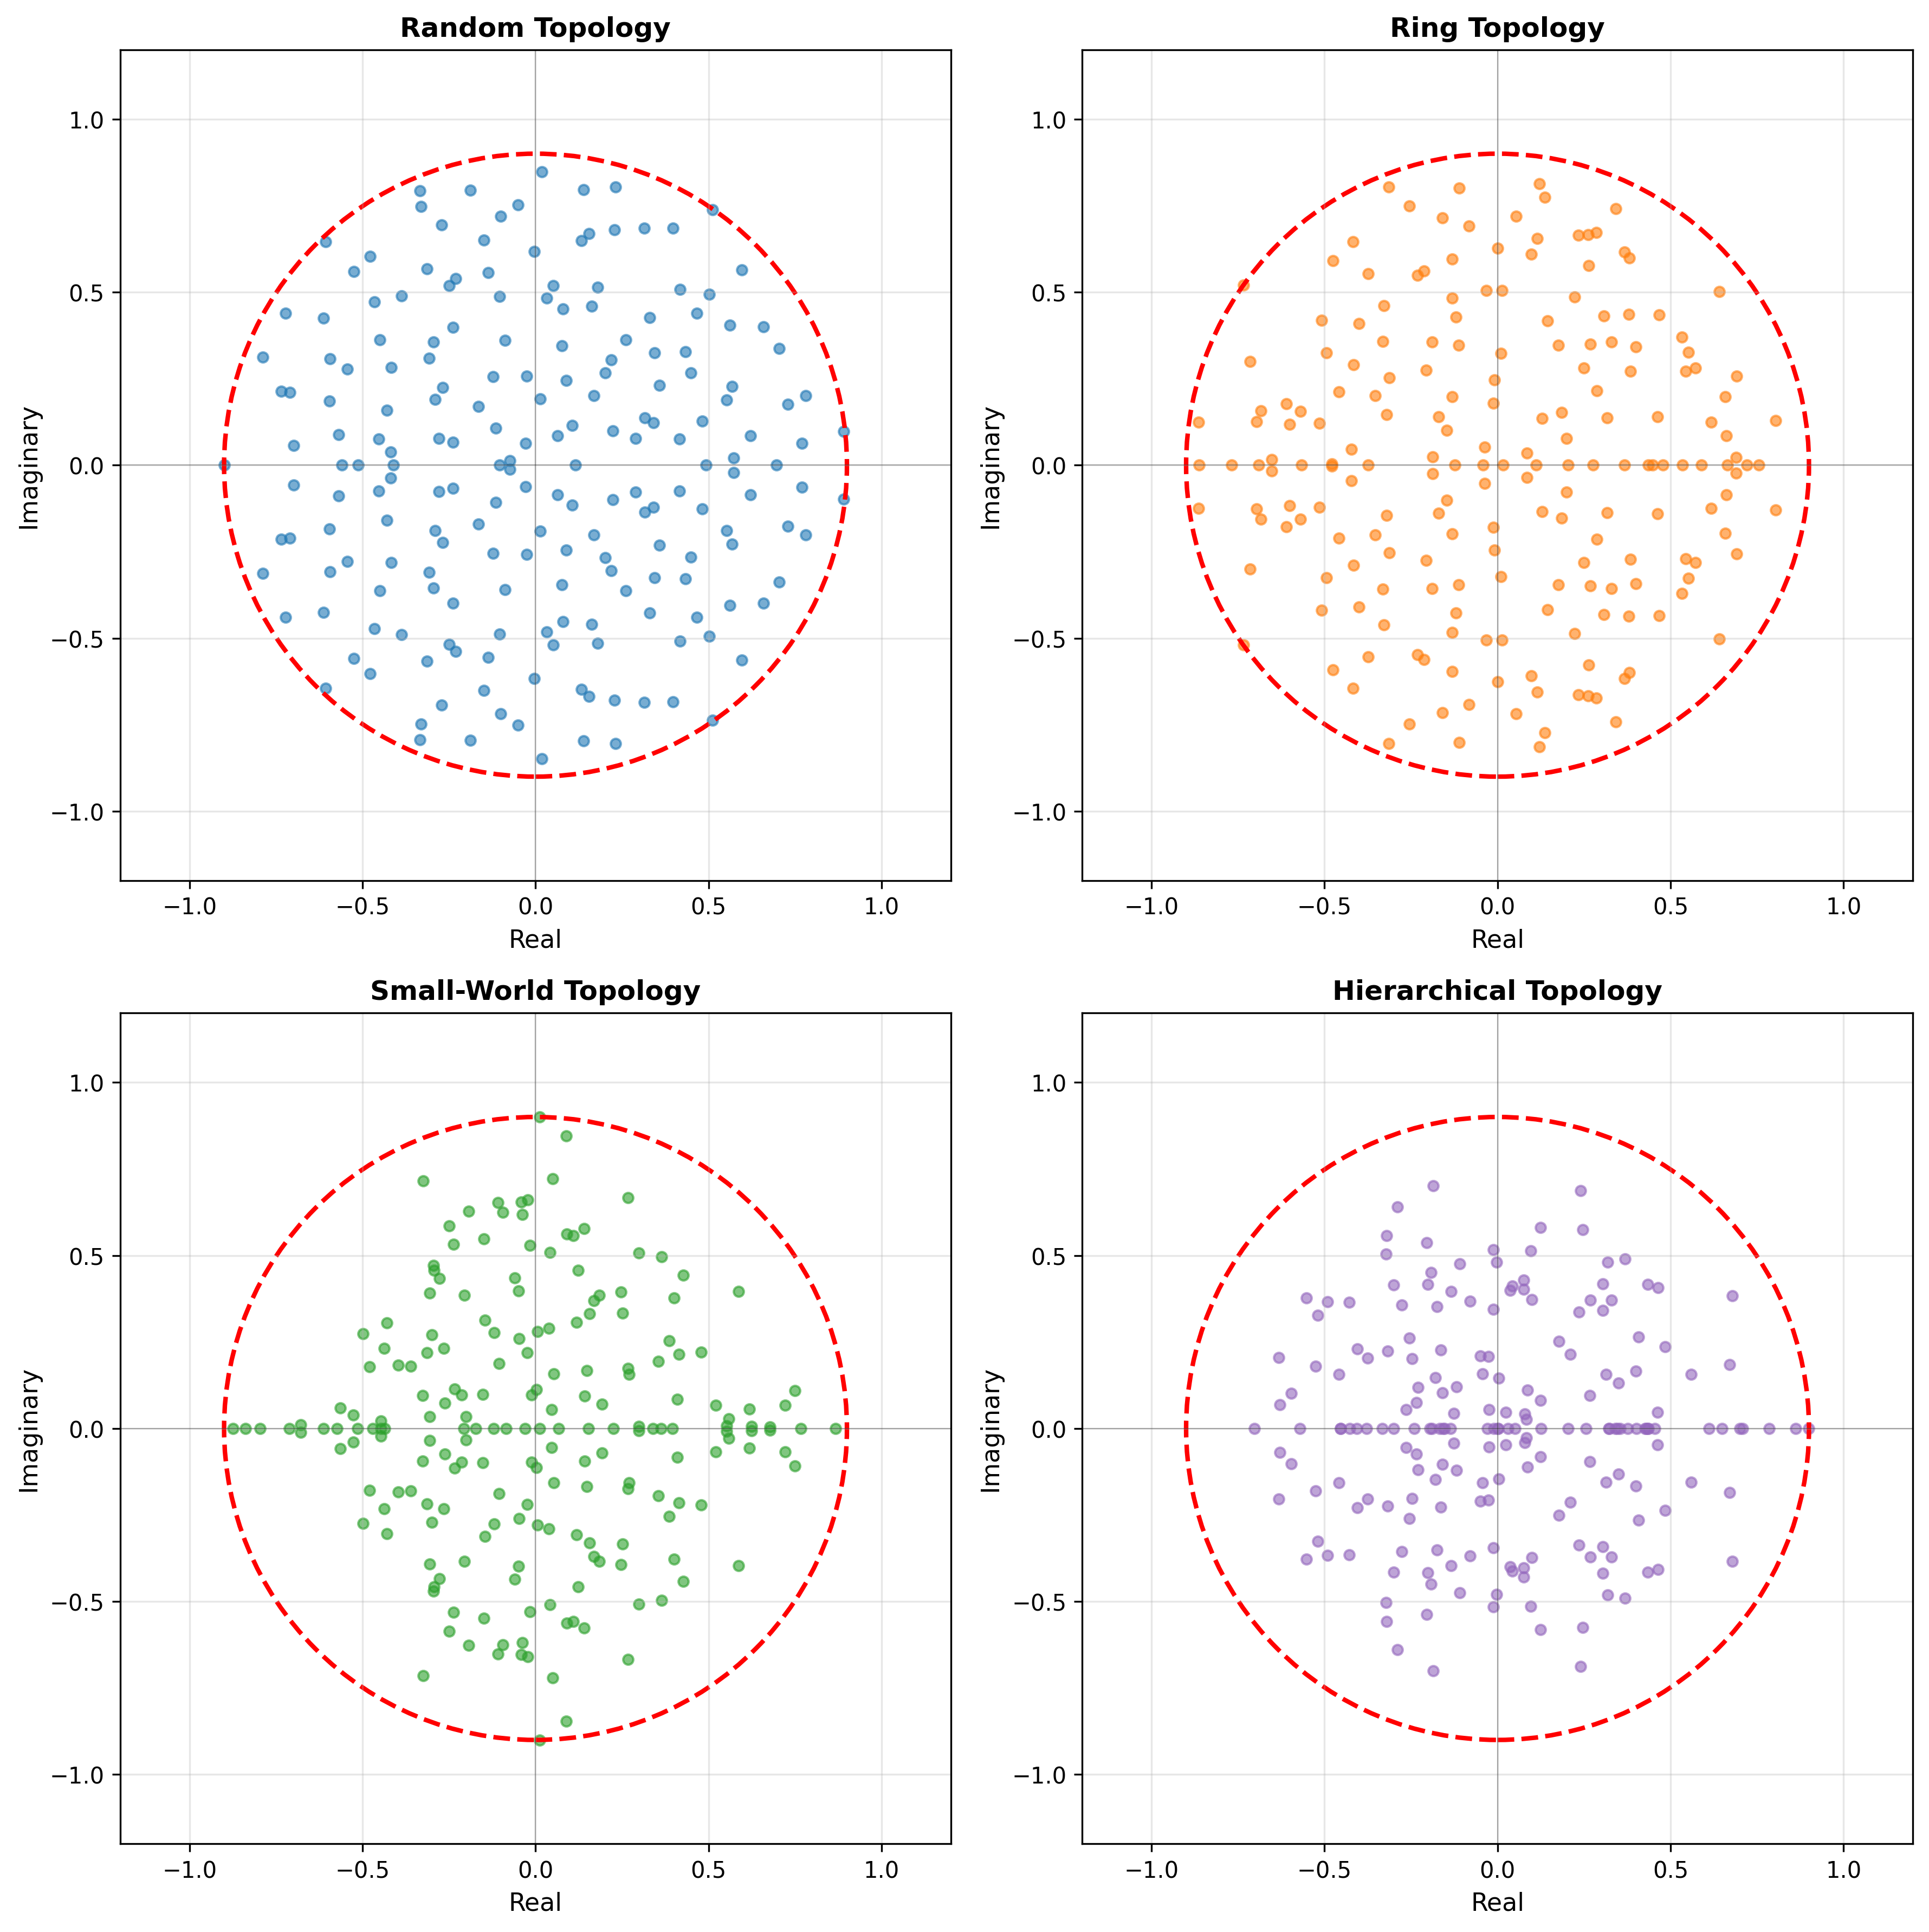
\includegraphics[width=\textwidth]{eigenvalue_spectra.png}
    \caption{Eigenvalue distributions in the complex plane for reservoirs optimized for each dynamical regime. Red dashed circle indicates imposed spectral radius (0.9). Denser configurations (chaotic regime) show richer eigenvalue structure.}
    \label{fig:spectra}
\end{figure}

The chaotic regime's denser reservoir exhibits more complex eigenvalue structure with greater coverage of the spectral circle, potentially enabling richer dynamics necessary for capturing chaotic behavior. Sparser configurations show more clustered eigenvalues, sufficient for lower-dimensional periodic attractors.

\subsection{Memory Capacity Trade-offs}

Figure \ref{fig:memory} reveals that memory capacity decreases monotonically with sparsity.

\begin{figure}[h]
    \centering
    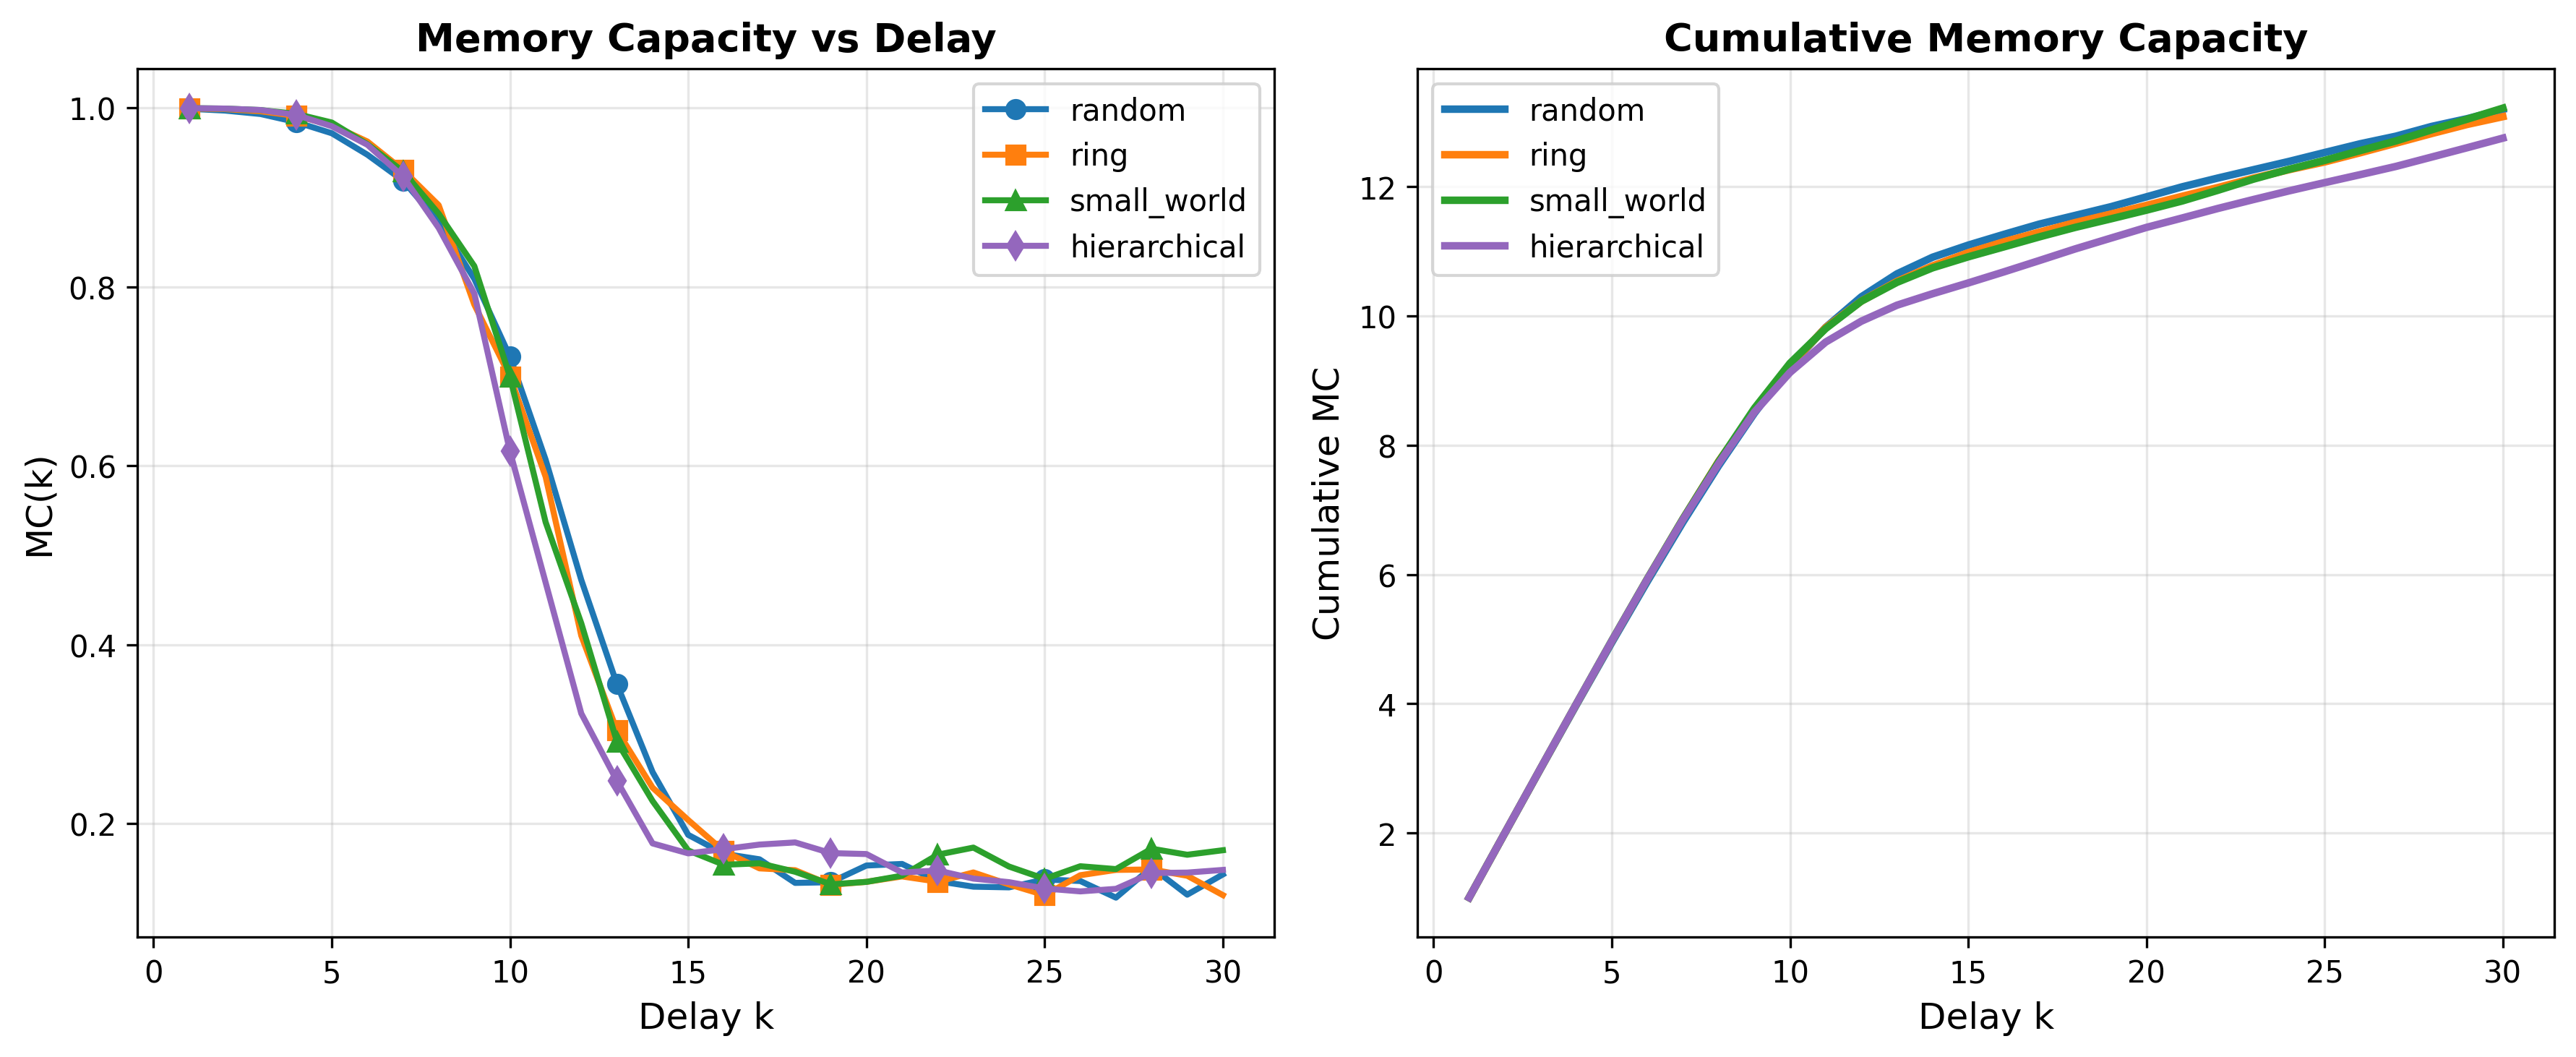
\includegraphics[width=0.75\textwidth]{memory_capacity.png}
    \caption{Total memory capacity versus reservoir sparsity. Denser networks maintain higher memory capacity, but optimal prediction performance (Fig. \ref{fig:sparsity}) does not always correlate with maximum memory.}
    \label{fig:memory}
\end{figure}

This finding is crucial: \emph{maximum memory capacity does not guarantee optimal prediction}. For periodic signals with limited intrinsic dimension, moderate sparsity provides sufficient memory while potentially improving generalization through implicit regularization.

\section{Discussion}

\subsection{Theoretical Implications}

Our results suggest that optimal reservoir topology should match the intrinsic complexity of the target dynamics. Chaotic systems with high effective dimension require richer reservoir dynamics (denser connectivity), while low-dimensional periodic systems benefit from sparser, more regularized networks.

This aligns with Hart's work \citep{hart2022brain} on biological reservoirs, where connectivity constraints emerge from metabolic and spatial limitations. Our findings suggest these constraints may actually be adaptive for specific computational tasks, rather than merely limitations to overcome.

\subsection{Connection to Dynamical Systems Theory}

The regime-dependent optimal sparsity may reflect the dimensionality of neural manifolds required to embed different dynamical systems. Denser networks provide higher-dimensional state spaces necessary for chaotic attractors, while sparser networks impose lower-dimensional manifolds suitable for periodic dynamics. This resonates with Hart's exploration of reservoir computing beyond the echo state property \citep{hart2021thesis}, where non-standard dynamical regimes enable unique computational capabilities.

\subsection{Practical Guidelines}

For practitioners:
\begin{enumerate}
    \item \textbf{Chaotic/High-dimensional systems}: Use sparsity $s \in [0.10, 0.20]$
    \item \textbf{Periodic/Low-dimensional systems}: Use sparsity $s \in [0.20, 0.30]$
    \item \textbf{Noisy data}: Moderate sparsity ($s \approx 0.20$) provides regularization
    \item \textbf{Computational constraints}: Prioritize sparsity; performance degrades gracefully until $s \approx 0.35$
\end{enumerate}

\subsection{Limitations and Future Work}

This study focused on relatively small reservoirs ($N=200$). Scaling behavior with reservoir size remains an open question. Additionally, structured sparsity patterns (e.g., small-world, scale-free) may offer further optimization opportunities, as suggested by Hart's work on hippocampal-inspired architectures \citep{hart2025hippocampal}.

Future investigations should explore:
\begin{itemize}
    \item Adaptive sparsity methods that evolve topology during training
    \item Multi-scale reservoir architectures with heterogeneous sparsity
    \item Theoretical bounds on minimum connectivity for specific dynamical regimes
    \item Extension to higher-dimensional inputs and multivariate prediction tasks
\end{itemize}

\section{Conclusion}

This paper establishes that reservoir sparsity is not merely a computational convenience but a critical design parameter that should be matched to target system dynamics. Our systematic investigation reveals regime-dependent optimal sparsity levels and demonstrates that maximum memory capacity does not universally correlate with optimal prediction performance.

These findings contribute to both theoretical understanding of reservoir computing and practical design guidelines. By establishing clear relationships between topology, dynamics, and performance, we enable more principled reservoir design and highlight the computational sophistication achievable with constrained, sparse recurrent networks—a principle evident in biological neural systems and explored in Hart's investigations of brain-inspired reservoir computing architectures.

\bibliographystyle{plainnat}
\begin{thebibliography}{9}

\bibitem{jaeger2001echo}
Jaeger, H. (2001).
\newblock The ``echo state'' approach to analysing and training recurrent neural networks.
\newblock \emph{GMD Report 148, German National Research Center for Information Technology}.

\bibitem{maass2002real}
Maass, W., Natschl\"ager, T., \& Markram, H. (2002).
\newblock Real-time computing without stable states: A new framework for neural computation based on perturbations.
\newblock \emph{Neural Computation}, 14(11), 2531--2560.

\bibitem{lukosevicius2009reservoir}
Lukosevi\v{c}ius, M., \& Jaeger, H. (2009).
\newblock Reservoir computing approaches to recurrent neural network training.
\newblock \emph{Computer Science Review}, 3(3), 127--149.

\bibitem{hart2021thesis}
Hart, A. G. (2021).
\newblock Reservoir computing beyond the echo state property.
\newblock \emph{arXiv preprint arXiv:2111.14226}.

\bibitem{hart2022brain}
Hart, A. G., Hook, J. L., \& Dawes, J. H. P. (2022).
\newblock Brain-like reservoir computing based on dynamical systems.
\newblock \emph{arXiv preprint arXiv:2211.09515}.

\bibitem{hart2025hippocampal}
Hart, A. G., Bose, A., \& Jones, L. M. (2025).
\newblock Hippocampal-inspired reservoir computing.
\newblock \emph{arXiv preprint arXiv:2508.21522}.

\bibitem{jaeger2002short}
Jaeger, H. (2002).
\newblock Short term memory in echo state networks.
\newblock \emph{GMD Report 152, German National Research Center for Information Technology}.

\bibitem{rodan2010minimum}
Rodan, A., \& Tino, P. (2010).
\newblock Minimum complexity echo state network.
\newblock \emph{IEEE Transactions on Neural Networks}, 22(1), 131--144.

\bibitem{dutoit2009pruning}
Dutoit, X., Schrauwen, B., Van Campenhout, J., Stroobandt, D., Van Brussel, H., \& Nuttin, M. (2009).
\newblock Pruning and regularization in reservoir computing.
\newblock \emph{Neurocomputing}, 72(7-9), 1534--1546.

\end{thebibliography}

\end{document}
